% !TeX program = xelatex
\documentclass{beamer}
\usepackage{etex} % fixes new-dimension error
%-------------- template --------------------------------------------------
\usetheme{metropolis}
\metroset{block=fill}
%\usetheme{Boadilla}

% Configuring the foot line
\setbeamertemplate{footline}
{
  \leavevmode%
  \hbox{%
  \begin{beamercolorbox}[wd=.4\paperwidth,ht=2.25ex,dp=1ex,center]{author in head/foot}%
    \usebeamerfont{author in head/foot}\insertshortauthor
  \end{beamercolorbox}%
  \begin{beamercolorbox}[wd=.5\paperwidth,ht=2.25ex,dp=1ex,center]{title in head/foot}%
    \usebeamerfont{title in head/foot}\insertsection
  \end{beamercolorbox}%
  \begin{beamercolorbox}[wd=.1\paperwidth,ht=2.25ex,dp=1ex,right]{date in head/foot}%
    \insertframenumber{} / \inserttotalframenumber\hspace*{2ex} 
  \end{beamercolorbox}}%
  \vskip0pt%
}
% No configuration symbols
\makeatother
\setbeamertemplate{navigation symbols}{}
%----------------------------------------------------------------------------
% context
\AtBeginSection[]
{
    \begin{frame}
        \frametitle{Table of Contents}
        \tableofcontents[currentsection]
    \end{frame}
}
\author[Renato Neves]{Renato Neves}

% logos of institutions
\titlegraphic{
  \begin{textblock*}{5cm}(7.8cm,7.45cm)
     
\includegraphics[scale=0.044]{images/uminho.png}\hspace*{.85cm}~%
  \end{textblock*}
  \begin{textblock*}{5cm}(9.8cm,7.45cm)
    
\includegraphics[scale=0.4]{images/haslab.pdf}
  \end{textblock*}
}

% no date
\date{}

%----------------------------------------------------------------------------
\usepackage{graphicx,amsmath}
\usepackage{stmaryrd} % cf. interleave
\usepackage{booktabs}
\usepackage{amscd}
\usepackage[absolute,overlay]{textpos} % this is for textblock
\usepackage{tikz}
\usetikzlibrary{arrows.meta, calc, fit, tikzmark}
\usepackage{pgfplots}
\usepackage{alltt}
\usepackage{listings}
\usepackage{proof}
\usepackage[all]{xy}
% temp
\newcommand{\blue}[1]{\textcolor{blue}{#1}}
\begin{document}

\title{Hybrid Programming}

\frame[plain]{\titlepage}

\section{Overview}

\begin{frame}{Last Lectures}
       
       Explored a simple language (\textsc{ccs}) and its semantics

       \bigskip
       Used it in the design of \alert{communicating} systems

       \bigskip
       Expanded this study to the \alert{timed} setting
       
       \bigskip
       Used results to save us all from zombies !!!

\end{frame}


\begin{frame}{Going beyond the timed setting}

        \begin{minipage}[0.3\textheight]{\textwidth}
        \begin{columns}[c]
                \begin{column}{0.45\textwidth}
                \scalebox{0.6}{
                  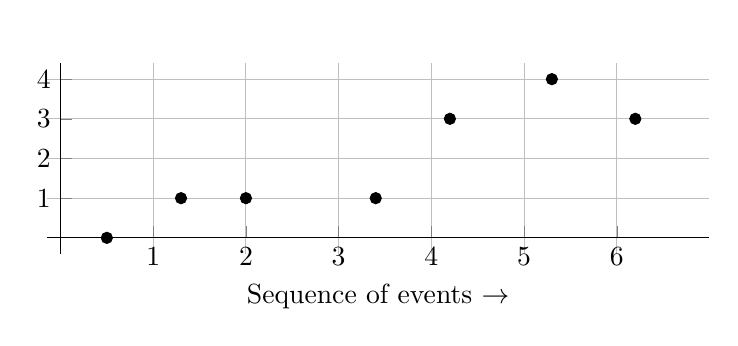
\begin{tikzpicture}
                   \begin{axis}[width=10cm, height=4cm, x axis line style={}, grid =
                     major, y axis line style={},
                     title={\textbf{}}, xlabel={\tikzmark{y1}\tikzmark{y2}Sequence
                     of events $\rightarrow$}, xtick =
                     {0,1,2,3,4,5,6}, xmax=7, axis lines*=center,
                     ytick={0,1,2,3,4,5,6},ylabel={},
                     xlabel near ticks, ylabel near ticks] \addplot [color=black,
                             only marks, domain = 0:5 ] 
                             coordinates {(0.5,0) (1.3,1) (2,1) (3.4,1) 
                             (4.2,3) (5.3,4) (6.2,3)};
                   \end{axis}
                  \end{tikzpicture}} 
                \end{column}
                \begin{column}{0.1\textwidth} 
                        \hspace{0.5cm} \textbf{+}                
                \end{column}
                \begin{column}{0.50\textwidth} 
                \scalebox{0.6}{ 
                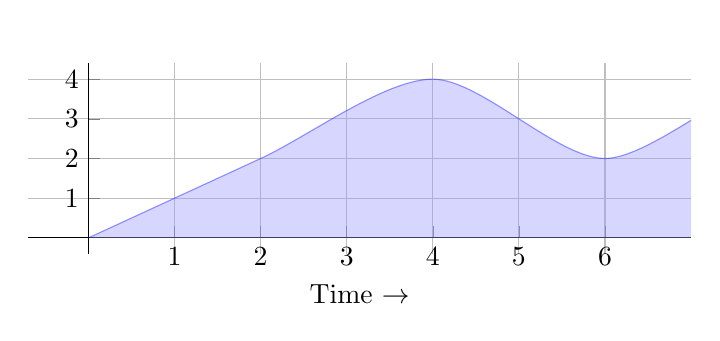
\begin{tikzpicture}
                \begin{axis}[width=10cm, height=4cm, x axis line style={}, grid =
                    major, y axis line style={},
                     title={\textbf{}}, xlabel={\tikzmark{x1}\tikzmark{x2}Time $\rightarrow$}				, xtick = {0,1,2,3,4,5,6} , xmax=7, axis lines*=center,
                     ytick={0,1,2,3,4,5,6}, ylabel={},
                     xlabel near ticks, ylabel near ticks] \addplot [color=blue, smooth,
                     domain = 0:5, fill = blue!40!white, opacity=0.4 ] coordinates {
                     (0,0) (2,2) (4,4) (6,2) (8,4) (8,0)};
                \end{axis}
                \end{tikzpicture}}
                \end{column}
        \end{columns}
        \end{minipage}

        \vspace{1.5cm}
        \begin{center}
                Computational devices now interact with \alert{arbitrary}
                physical processes (and not just time)
        \end{center}

        \begin{tikzpicture}[overlay,remember picture,
                box/.style = {rounded corners},
                pin edge={-Stealth,thick, red}]
                \coordinate (x1) at ($({pic cs:x1})+(6ex, -10ex)$);
                \coordinate (x2) at ($({pic cs:x2})+(7ex, 0ex)$);
                \node[semitransparent,
                     fit=(x1) (x2),
                     pin=below:\tiny{Described via differential equations}]  {};
        \end{tikzpicture} 

        \begin{tikzpicture}[overlay,remember picture, box/.style
                = {rounded corners}, pin edge={-Stealth,thick, red}] 
                \coordinate (y1) at
                     ($({pic cs:y1})+(7ex, -10.6ex)$); 
                \coordinate (y2) at ($({pic cs:y2})+(7ex,-2ex)$); 
                \node[semitransparent, fit=(y1) (y2),
                     pin=below:\tiny{Described via classical methods of computation}]
                {};
        \end{tikzpicture}

\end{frame}

\begin{frame}{Which language ?}

        This time we explore a simple, \alert{imperative} language

        \bigskip
        No concurrency and no communication

        \dots\ 
        languages with such features are still underdeveloped

        \bigskip
        Perhaps some of you would like to improve them ;-)

\end{frame}

\begin{frame}{The hybrid while-Language}

        \vspace{0.7cm}
	\begin{block}{Linear Terms}
	$\mathtt{LTerm} ::= \tikzmark{r1} \mathtt{r} \tikzmark{r2} \mid \mathtt{r \cdot t}
        \mid \tikzmark{u1} \mathtt{x} \tikzmark{u2} \mid \mathtt{t + s}$
	\end{block}

	\vspace{1cm}
	\begin{block}{Atomic Programs}
	$\mathtt{At} ::= \mathtt{x := t} \mid
	\mathtt{x'_1 = t_1, \dots, x'_n = t_n \> \> \tikzmark{d1}\blue{for}\tikzmark{d2} 
	\> \> t }$
	\end{block}

	\vspace{1cm}
	\begin{block}{Programs}
	$\mathtt{Prog} ::= \mathtt{a} \mid
	\mathtt{p \> \blue{;} \> q} \mid
	\mathtt{\blue{if} \> b \> \blue{then} \> p \> \blue{else} \> q} \mid
	\mathtt{\blue{while} \> b \> \blue{do} \> \{ \> p \> \}}$
	\end{block}

	\begin{tikzpicture}[overlay,remember picture,
	box/.style = {rounded corners},
	pin edge={-Stealth,thick, red}]
	\coordinate (r1) at ($({pic cs:r1})+(-0.2ex, 1.5ex)$);
	\coordinate (r2) at ($({pic cs:r2})+(0.2ex, -0.5ex)$);
	\node[semitransparent,
	     fit=(r1) (r2),
	     pin=below:\tiny{real number}]  {};
	\end{tikzpicture}

	\begin{tikzpicture}[overlay,remember picture,
	box/.style = {rounded corners},
	pin edge={-Stealth,thick, red}]
	\coordinate (u1) at ($({pic cs:u1})+(-0.2ex, 1.5ex)$);
	\coordinate (u2) at ($({pic cs:u2})+(0.2ex,-0.5ex)$);
	\node[semitransparent,
	     fit=(u1) (u2),
	     pin=below:\tiny{variable}]  {};
	\end{tikzpicture}

	\begin{tikzpicture}[overlay,remember picture,
	box/.style = {rounded corners},
	pin edge={-Stealth,thick, red}]
	\coordinate (d1) at ($({pic cs:d1})+(-0.2ex, 1.5ex)$);
	\coordinate (d2) at ($({pic cs:d2})+(0.2ex,-0.5ex)$);
	\node[semitransparent,
	     fit=(d1) (d2),
	     pin=below:\tiny{"run" the system of differential 
	     equations for $\mathtt{t}$ seconds}]  {};
	\end{tikzpicture}

\end{frame}

\begin{frame}{Overview}

        We study a while-language without differential equations

        \bigskip
        Then move to the hybrid case and see how semantics aids in the analysis
        of hybrid programs

        \bigskip
        Throughout this journey, we will:
        \begin{itemize}
                \item write implementations in \textsc{haskell}
                \item do analyses in \textsc{lince}
        \end{itemize}
\end{frame}

\section{Semantics}

\begin{frame}{A language of linear terms and its semantics}

        \begin{block}{Linear terms}
	$\mathtt{LTerm} ::= \mathtt{r} \mid \mathtt{r \cdot t}
        \mid \mathtt{x}  \mid \mathtt{t + s }$
	\end{block}

        $\sigma : X \to \mathbb{R}$ denote a \alert{memory}

        $\langle \mathtt{t},\sigma \rangle \Downarrow \mathtt{r}$
        means that $\mathtt{t}$ outputs $\mathtt{r}$ if current memory is
        $\sigma$

        \[
                \infer[(\text{var})]{\langle \mathtt{x}, \sigma \rangle 
                \Downarrow \sigma(\mathtt{x})}{} \qquad \qquad
                \infer[(\text{con})]{\langle \mathtt{r}, \sigma \rangle 
                \Downarrow \mathtt{r}}{}
        \] \vspace{0.1cm}        
        \[        
                \infer[(\text{scl})]{  
                        \langle \mathtt{s} \cdot \mathtt{t}, \sigma \rangle \Downarrow 
                        \mathtt{s \cdot r}
                        }{
                        \langle \mathtt{t}, \sigma \rangle \Downarrow \mathtt{r}
                } \qquad \qquad
                \infer[(\text{add})]{  
                        \langle \mathtt{t_1} + \mathtt{t_2}, \sigma \rangle \Downarrow 
                        \mathtt{r_1 + r_2}
                        }{
                        \langle \mathtt{t_1}, \sigma \rangle \Downarrow \mathtt{r_1} \qquad
                        \langle \mathtt{t_2}, \sigma \rangle \Downarrow \mathtt{r_2}
                }
        \]
\end{frame}        


\begin{frame}{The semantics at work}
        $\mathtt{x + 2 \cdot y}$ corresponds to the 
        \alert{syntax} tree
        \[
                \xymatrix@C=10pt@R=10pt{
                        & (+) \ar[dl] \ar[dr]  & \\
                        \mathtt{x} & & \mathtt{(2\ \cdot)} \ar[d] \\
                        & & \mathtt{y} 
                }
        \]

        \vspace{0.4cm}
        $\sigma(\mathtt{x}) = 3$ and $\sigma(\mathtt{y}) = 4$
        yield the "\alert{semantic} tree"
        \[
                \infer{\langle \mathtt{ x + 2 \cdot y}, \sigma \rangle \Downarrow 
                \mathtt{11} }{
                        \langle \mathtt{x}, \sigma \rangle \Downarrow \mathtt{3} 
                        \qquad \qquad
                        \infer{\langle \mathtt{2 \cdot y}, \sigma \rangle \Downarrow 8}{
                        \langle \mathtt{y}, \sigma \rangle \Downarrow 4}
                }
        \]
\end{frame}

\begin{frame}{Exercises}
        Write down the corresponding derivation trees for
        \begin{itemize}
                \item $\mathtt{2 \cdot x + 2 \cdot y}$
                \item $\mathtt{3 \cdot (2 \cdot x) + 2 \cdot (y + z)}$ 
        \end{itemize}

        \pause
        \bigskip
        Boring computations? If so why not implement the semantics?
\end{frame}

\begin{frame}{A language of Boolean terms and its semantics}

        \begin{block}{Boolean terms}
        $\mathtt{BTerm} ::= \mathtt{t \leq t} \mid \mathtt{b \wedge b}
        \mid \mathtt{\neg b}$
	\end{block}
        $\langle \mathtt{b},\sigma \rangle \Downarrow
        \mathtt{v}$ tells that $\mathtt{b}$ outputs
        $\mathtt{v}$ if the memory is $\sigma$

        \[
                \infer[(\text{leq})]
                { 
                        \langle \mathtt{t_1 \leq t_2}, \sigma \rangle \Downarrow \mathtt{tt} 
                }
                {
                        \langle \mathtt{t_1}, \sigma \rangle \Downarrow \mathtt{r_1} \qquad
                        \langle \mathtt{t_2}, \sigma \rangle \Downarrow \mathtt{r_2}
                        \qquad \mathtt{r_1 \leq r_2}
                } 
        \] 
        \vspace{0.1cm}
        \[
                \infer[(\text{gtr})]
                { 
                        \langle \mathtt{t_1 \leq t_2}, \sigma \rangle \Downarrow \mathtt{ff} 
                }
                {
                        \langle \mathtt{t_1}, \sigma \rangle \Downarrow \mathtt{r_1} \qquad
                        \langle \mathtt{t_2}, \sigma \rangle \Downarrow \mathtt{r_2}
                        \qquad \mathtt{r_1 \not \leq r_2}
                }
        \]
        \vspace{0.1cm}
        \[        
                \infer[(\text{not})]{  
                        \langle \mathtt{\neg \mathtt{b}}, \sigma \rangle \Downarrow 
                        \mathtt{\neg v}
                        }{
                        \langle \mathtt{b}, \sigma \rangle \Downarrow \mathtt{v}
                } \qquad \qquad
                \infer[(\text{and})]{  
                        \langle \mathtt{b_1} \wedge \mathtt{b_2}, \sigma \rangle \Downarrow 
                        \mathtt{v_1 \wedge v_2}
                        }{
                        \langle \mathtt{b_1}, \sigma \rangle \Downarrow \mathtt{v_1} \qquad
                        \langle \mathtt{b_2}, \sigma \rangle \Downarrow \mathtt{v_2}
                }
        \]
\end{frame}        


\begin{frame}{A while-language and its semantics}
	\begin{block}{Programs}
	        $\mathtt{Prog} \ni \mathtt{x := t} \mid
	        \mathtt{p \> \blue{;} \> p} \mid
	        \mathtt{\blue{if} \> b \> \blue{then} \> p \> \blue{else} \> p} \mid
	        \mathtt{\blue{while} \> b \> \blue{do} \> \{ \> p \> \}}$
        \end{block} 
        
        \scalebox{0.95}{
        \begin{minipage}{1\linewidth}
        \[
                \infer[(\text{asg})]{
                        \langle \mathtt{x := t}, \sigma \rangle \Downarrow 
                        \sigma[\mathtt{r} / \mathtt{x}]
                }{
                       \langle \mathtt{t}, \sigma \rangle \Downarrow \mathtt{r}
                } \hspace{1cm}
                \infer[(\text{seq})]{
                        \langle \mathtt{p \> \blue{;} \> q}, \sigma \rangle \Downarrow \sigma''
                }{
                        \langle \mathtt{p}, \sigma \rangle \Downarrow \sigma' \qquad
                        \langle \mathtt{q}, \sigma' \rangle \Downarrow \sigma'' 
                }
        \]\vspace{0.001cm}
        \[\hspace{-0.6cm}
                \infer[(\text{if1})]{
                        \langle \mathtt{\blue{if} \> b \> \blue{then} \> \> p \> \blue{else} \> q}, 
                        \sigma \rangle \Downarrow \sigma'
                }{
                        \langle \mathtt{b}, \sigma \rangle \Downarrow \mathtt{tt} \qquad
                        \langle \mathtt{p}, \sigma \rangle \Downarrow \sigma'
                } \hspace{1cm} 
                \infer[(\text{if2})]{
                        \langle \mathtt{\blue{if} \> b \> \blue{then} \> \> p \> \blue{else} \> q}, 
                        \sigma \rangle \Downarrow \sigma'
                }{
                        \langle \mathtt{b}, \sigma \rangle \Downarrow \mathtt{ff} \qquad
                        \langle \mathtt{q}, \sigma \rangle \Downarrow \sigma'
                } 
        \]\vspace{0.001cm}
        \[
                \infer[(\text{wh1})]{
                        \langle \mathtt{\blue{while} \> b \> \blue{do} \> \{ \> p \> \}}, \sigma \rangle
                        \Downarrow \sigma''
                }{
                        \langle \mathtt{b}, \sigma \rangle \Downarrow \mathtt{tt} \qquad
                        \langle \mathtt{p}, \sigma \rangle \Downarrow \sigma' \qquad
                        \langle \mathtt{\blue{while} \> b \> \blue{do} \> \{ \> p \> \}}, \sigma'
                        \rangle \Downarrow \sigma'' 
                }
        \]\vspace{0.001cm}
        \[
                \infer[(\text{wh2})]{
                        \langle \mathtt{\blue{while} \> b \> \blue{do} \> \{ \> p \> \}}, \sigma \rangle
                        \Downarrow \sigma
                }{
                        \langle \mathtt{b}, \sigma \rangle \Downarrow \mathtt{ff}
                }
        \]
        \end{minipage}
        }
\end{frame}


\begin{frame}{The semantics at work}
        $\mathtt{x := x + 1 \> \blue{;} \> x := x + 2}$ corresponds to the 
        `\alert{syntax} tree'
        \[
                \xymatrix@C=10pt@R=10pt{
                        & (\> ; \>) \ar[dl] \ar[dr]  & \\
                        \mathtt{x := x + 1} & & \mathtt{x := x + 2} 
                }
        \]

        \vspace{0.4cm}
        Memory $\sigma = x \mapsto 3$ yields the `\alert{semantic} tree'
        \[
                \infer{
                        \langle \mathtt{ x := x + 1 \> \blue{;} \> x := x + 2 }, \mathtt{x \mapsto 3}
                        \rangle \Downarrow \mathtt{x \mapsto 6}
                }{
                        \infer{
                                \langle \mathtt{x := x +1}, \mathtt{x \mapsto 3} \rangle 
                                \Downarrow \mathtt{x \mapsto 4}
                        }{
                                \langle \mathtt{x + 1}, \mathtt{x \mapsto 3} \rangle \Downarrow
                                \mathtt{4}
                        }\qquad \qquad                        
                        \infer{
                                \langle \mathtt{x := x + 2}, \mathtt{x \mapsto 4} \rangle 
                                \Downarrow \mathtt{x \mapsto 6}
                        }{
                                \langle \mathtt{x + 2}, \mathtt{x \mapsto 4} \rangle \Downarrow
                                \mathtt{6}
                        }
                }
        \]
\end{frame}


\end{document}

